\documentclass{article}
\usepackage[utf8]{inputenc}
\usepackage{graphicx}
\usepackage{amsmath}

\title{Intelligens Fejlesztőeszkozok - 4. beadandó}
\author{Sándor Burian}
\date{Szeptember 2022}

\begin{document}

\maketitle

\section{feladat}

Intervallum felező módszerrel 
\begin{equation}
    5x-4 = sin(tanh(-3x+2)); [-10,10] intervallumon 
\end{equation}


\begin{multline}
\\
f(x) = 5x-4-sin(tanh(-3x+2)) \\
a_1 = -10 \\
b_1 = 10\\
f(a_1)=f(-10)=-50-4-sin(tanh(32)) = -54 - 0,017452406 = -54,017452406 \\
f(b_1)=f(10) = 50-4 - sin(tanh(-28)) = 46 - (-0,017452406) = 46,017452406 \\
\\
\Rightarrow f(a)f(b)<0 \Rightarrow intervallumfelezes: \dfrac{a+b}{2} \Rightarrow \frac{10+(-10)}{2} = 0 \\
\end{multline}

\begin{multline}
\\
f(0) = -4-sin(tanh(2)) = -4-0,016824661 = -4,016824661\\
a_2 = (a_1 + b_1)/2 = 0; f(a_2) < 0
b_2 = b_1=10\\
f(b_2) >0\\
f(\dfrac{a_2+b_2}{2}) = f(5) = 25-4-sin(tanh(-13)) = 21,017452406 \\
b_3 = 5\\
f(b_3) > 0 \\
a_3 = a_2 = 0 \\
f(a_3)<0\\
f(0)f(5) < 0 \\
f(2.5) = 12.5-4-sin=tanh(-5.5)) = 8,517451824 \\
...\\
f(\dfrac{a_23 + b_23}{2}) = f(0,798685552) = 0,000000094 \\
\Rightarrow x = 0,798685552\\
\end{multline}

Julia kódként:

\begin{verbatim}
f(x)=5*x-4-sin(tanh(-3*x+2))
a=-10
b=10
ϵ=1e-7 #(10^(-7))

while true
    global a,b
    c=(a+b)/2
    println("x= ",c)
    println("f(x)= ",f(c))
    println()
    if sign(f(c))==sign(f(a))
        a=c
    end
    if sign(f(c))==sign(f(b))
        b=c
    end
    if abs(f(c))<ϵ
        break
    end
end
\end{verbatim}

Logok:

\begin{verbatim}
x= 0.0  
f(x)= -4.821494815516438

x= 5.0
f(x)= 21.841470984802374

x= 2.5
f(x)= 9.341452936704993

x= 1.25
f(x)= 3.0583686122902405

x= 0.625
f(x)= -0.9990327572022525

x= 0.9375
f(x)= 1.3092437102511458

x= 0.78125
f(x)= 0.2310697309851627

x= 0.703125
f(x)= -0.37564942969465204

x= 0.7421875
f(x)= -0.06813638549908974

x= 0.76171875
f(x)= 0.08270992936515631

x= 0.751953125
f(x)= 0.007575155275291817

x= 0.7470703125
f(x)= -0.030211616196670926

x= 0.74951171875
f(x)= -0.011300580891388218

x= 0.750732421875
f(x)= -0.001858251535921368

x= 0.7513427734375
f(x)= 0.0028595732281952724

x= 0.75103759765625
f(x)= 0.0005009404338206236

x= 0.750885009765625
f(x)= -0.0006785857483954938

x= 0.7509613037109375
f(x)= -8.880519482826199e-5

x= 0.7509994506835938
f(x)= 0.0002060719865843441

x= 0.7509803771972656
f(x)= 5.863448746595834e-5

x= 0.7509708404541016
f(x)= -1.5085080807220042e-5

x= 0.7509756088256836
f(x)= 2.1774771550742145e-5

x= 0.7509732246398926
f(x)= 3.3448624267573557e-6

x= 0.7509720325469971
f(x)= -5.8701049265030836e-6

x= 0.7509726285934448
f(x)= -1.2626201839338602e-6

x= 0.7509729266166687
f(x)= 1.0411213878791514e-6

x= 0.7509727776050568
f(x)= -1.107493314278507e-7

x= 0.7509728521108627
f(x)= 4.6518604487899573e-7

x= 0.7509728148579597
f(x)= 1.7721836090278664e-7

x= 0.7509727962315083
f(x)= 3.323451580605763e-8
\end{verbatim}

Ábrázolva:

\includegraphics[scale=1]{../plot_2.png} 

\section{feladat}

\begin{equation}
x+3= e^{sin(x+3)}
\end{equation}

Intervallum felező módszerrel [-10,10] között.

Matematikai levezetés hasonlatos.

Julia kód:

\begin{verbatim}
f(x)=x+3-ℯ^(sin(x+3))
a=-10
b=10
ϵ=1e-7 #(10^(-7))

while true
    global a,b
    c=(a+b)/2
    println("x= ",c)
    println("f(x)= ",f(c))
    println()
    if sign(f(c))==sign(f(a))
        a=c
    end
    if sign(f(c))==sign(f(b))
        b=c
    end
    if abs(f(c))<ϵ
        break
    end
end
\end{verbatim}

Logok:

\begin{verbatim}
x= 0.0  
f(x)= 1.848437163485465

x= -5.0
f(x)= -2.402807126123528 

x= -2.5
f(x)= -1.1151462964420837

x= -1.25
f(x)= -0.9250978172453692

x= -0.625
f(x)= 0.3739240078773549 

x= -0.9375
f(x)= -0.35209068903115126  

x= -0.78125
f(x)= -0.0008356627438894648

x= -0.703125
f(x)= 0.18456173681073818   

x= -0.7421875
f(x)= 0.0912498148899128

x= -0.76171875
f(x)= 0.04503881542828969

x= -0.771484375
f(x)= 0.022057630510200266

x= -0.7763671875
f(x)= 0.010599761786235007

x= -0.77880859375
f(x)= 0.004879214512186092

x= -0.780029296875
f(x)= 0.0020210634445905207

x= -0.7806396484375
f(x)= 0.0005925217794442439

x= -0.78094482421875
f(x)= -0.00012161518258224646

x= -0.780792236328125
f(x)= 0.00023544213054549346

x= -0.7808685302734375
f(x)= 5.691068110946773e-5

x= -0.7809066772460938
f(x)= -3.23529490668939e-5

x= -0.7808876037597656
f(x)= 1.2278691452927148e-5

x= -0.7808971405029297
f(x)= -1.0037172450960696e-5

x= -0.7808923721313477
f(x)= 1.1207485899333847e-6

x= -0.7808947563171387
f(x)= -4.458214657887538e-6

x= -0.7808935642242432
f(x)= -1.668733716098103e-6

x= -0.7808929681777954
f(x)= -2.739927333905712e-7

x= -0.7808926701545715
f(x)= 4.233778856388426e-7

x= -0.7808928191661835
f(x)= 7.469256546599468e-8
\end{verbatim}

Ábrázolva:

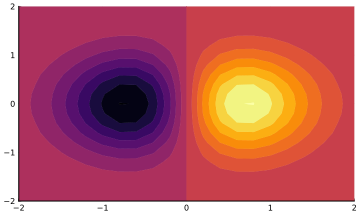
\includegraphics[scale=1]{../plot_3.png} 

\section{feladat}

\begin{equation}
6x+3 = tanh(tan(cos(-4x^{2}-3)))
\end{equation}

[-10,10] tartományon, Húr módszerrel

Húr engyelete:
\begin{multline}
a_0 = -10\\
x_0 = 10\\
f(-10)=-60+3-tanh(tan(cos(-403))) = -57.01276453\\
f(10) = 60+3-tanh(tan(cos(-403))) = 62.98723547\\
\end{multline}

innen 
\begin{multline}
x_{n+1} = a - \dfrac{x_n - a}{f(x_n) - f(a)} \dot{•} f(a)\\
f(x_n) \lt \epsilon \Rightarrow leall \Rightarrow x_n
\end{multline}

Julia kód:

\begin{verbatim}
f(x)=6*x+3-tanh(tan(cos(-4*x^2-3)))
a=-10
x=10
ϵ=1e-7

while true
    global x
    x=a-f(a)*(x-a)/(f(x)-f(a))
    println("x= ",x)
    println("f(x)= ",f(x))
    println()
    if abs(f(x))<ϵ
        break
    end
end
\end{verbatim}

logok

\begin{verbatim}
x= -0.3946673776396814
f(x)= 1.473222596433957

x= -0.6340843608639908    
f(x)= -0.7005580211701712 

x= -0.518834024842656     
f(x)= 0.475196224620007   

x= -0.5963702836862499    
f(x)= -0.29263090201165215

x= -0.5483789490399076    
f(x)= 0.19549112038083016 

x= -0.5803310204365939    
f(x)= -0.1252049477592092 

x= -0.5598223266568301
f(x)= 0.08271525237683225

x= -0.5733517486254289
f(x)= -0.05364104222537219

x= -0.564569711701985
f(x)= 0.035233678627016984

x= -0.5703345962277488
f(x)= -0.022957362273294757

x= -0.5665768482960285
f(x)= 0.015039215196470612

x= -0.5690378817376001
f(x)= -0.009817990684844624

x= -0.5674309813764502
f(x)= 0.006424128784621008

x= -0.5684822946895061
f(x)= -0.004197205014267735

x= -0.5677953690318347
f(x)= 0.002744922160006602

x= -0.568244588846385
f(x)= -0.001794004529417248

x= -0.5679509821710642
f(x)= 0.0011730000376027339

x= -0.5681429513807323
f(x)= -0.0007667509786616344

x= -0.5680174658453687
f(x)= 0.0005012887629938789

x= -0.5680995054428433
f(x)= -0.0003276959548840219

x= -0.5680458752817863
f(x)= 0.0002142334239423893

x= -0.5680809362282222
f(x)= -0.00014004957144803099

x= -0.5680580159837305
f(x)= 9.15567689105945e-5

x= -0.5680729999652794
f(x)= -5.98535484045426e-5

x= -0.5680632044536296
f(x)= 3.912869655703366e-5

x= -0.568069608173257
f(x)= -2.557978649297965e-5

x= -0.5680654218377033
f(x)= 1.6722493205334477e-5

x= -0.5680681586059535
f(x)= -1.0932096461913066e-5

x= -0.5680663694815777
f(x)= 7.146723589424031e-6

x= -0.5680675390994843
f(x)= -4.672074870593068e-6

x= -0.5680667744773746
f(x)= 3.054309705152747e-6

x= -0.5680672743393593
f(x)= -1.9967148497945786e-6

x= -0.5680669475611424
f(x)= 1.3053267006735148e-6

x= -0.5680671611882016
f(x)= -8.533403115240645e-7

x= -0.5680670215322934
f(x)= 5.57860228067586e-7

x= -0.5680671128305423
f(x)= -3.6469388708937345e-7

x= -0.5680670531454961
f(x)= 2.3841391838530512e-7

x= -0.5680670921638242
f(x)= -1.5586001317346998e-7

x= -0.5680670666560967
f(x)= 1.0189147403583121e-7

x= -0.5680670833314441
f(x)= -6.66102302204763e-8
\end{verbatim}

árbrázolva:

\includegraphics[scale=1]{../plot_4.png} 

\section{feladat}
\begin{equation}
x+2 = x^{3}
\end{equation}

[-10,10] tartományon, Newton-Raphson módszerrel

\begin{multline}
x_{n+1} = x_n - \frac{f(x_n)}{f'(x_n)-f(a)} \dot{•} f(a)\\
\end{multline}

ahol jelen esetben

\begin{multline}
f(x) = x+2 - x^{3}\\
f'(x) = 1-3x^{2}\\
\end{multline}

Julia kód:

\begin{verbatim}
f(x)=x+2-x^3
df(x)=1-3*x^2

x=-10
ϵ=1e-7

while true
    global x
    x=x-f(x)/df(x)
    println("x= ",x)
    println("f(x)= ",f(x))
    println()
    if abs(f(x))<ϵ
        break
    end
end
\end{verbatim}

Logok:

\begin{verbatim}
x= -6.682274247491639  
f(x)= 293.6999085590051

x= -4.473312792869828   
f(x)= 87.04003516198537 

x= -2.9988472242547655  
f(x)= 25.970039789119255

x= -1.999201900879969   
f(x)= 7.991224730944533 

x= -1.2720939925431056  
f(x)= 2.7864379244631436

x= -0.5492206014655907  
f(x)= 1.6164480962034022

x= -17.551900926196666  
f(x)= 5391.648634395187 

x= -11.711775501850084  
f(x)= 1596.741938527522 

x= -7.821998670703618
f(x)= 472.75653358358846

x= -5.232275467424355
f(x)= 140.01019468202122

x= -3.506526815777292
f(x)= 41.608781234980135

x= -2.3470941558915683
f(x)= 12.58269777701162

x= -1.5366954902088426
f(x)= 4.092107996851008

x= -0.864126976223906
f(x)= 1.7811299712985802

x= 0.572098718429206
f(x)= 2.3848525564336365

x= -131.12099781689727
f(x)= 2.2541969650863465e6

x= -87.4156545880499
f(x)= 667901.0175286231

x= -58.27955805586903
f(x)= 197890.64076094175

x= -38.8566558177144
f(x)= 58630.4649589283

x= -25.909715855150342
f(x)= 17369.62909815448

x= -17.280731383904506
f(x)= 5145.154818537878

x= -11.53112653863139
f(x)= 1523.7267835392222

x= -7.701711255066577
f(x)= 451.13573733453586

x= -5.152188160809331
f(x)= 133.61286731020152

x= -3.4530383049803026
f(x)= 39.71917254207688

x= -2.3107118145696806
f(x)= 12.027077638259073

x= -1.5098765713570435
f(x)= 3.9322302087075345

x= -0.8364551305833876
f(x)= 1.7487767118602822

x= 0.7548296498241522
f(x)= 2.3247520206776104

x= 4.032343923946572
f(x)= -59.5327518144143

x= 2.7863516954778125
f(x)= -16.84620236002299

x= 2.030620667549976
f(x)= -4.342481805448995

x= 1.6487049095196127
f(x)= -0.8328507392434155

x= 1.5322985411023986
f(x)= -0.06544468594788322

x= 1.5214701702523892
f(x)= -0.0005377329652014318

x= 1.5213797130880249
f(x)= -3.734754283613029e-8
\end{verbatim}

Mivel az utolsó kapott érték az intervallumon belül van így elfogadjuk.


\section{feladat}
\begin{equation}
f(x)= sin(x-5)
\end{equation}

[-10,10] tartományon, Fixpont iterációval kiindulópont x_0 = 5,5

\begin{multline}
f(x)=0\\
sin(x-5)=0\\
\end{multline}

a függvény x+g(x) alakban:

\begin{multline}
sin(x-5)=x-5-\frac{(x-5)^{3}}{3!}+\frac{(x-5)^{5}}{5!} - \frac{(x-5)^{7}}{7!} + ....
x_{0} = 5.5\\
x_{1} = g(x_0) = 5 + 0.5-\dfrac{0.125}{6}+\dfrac{0.03125}{120}-\dfrac{0.0078125}{5040} = 5,020574467\\
x_2 = g(x_1) = 5,000001452\\
x_3 = g(x_2) = 5\\
x_4 = g(x_3) = 5\\
\end{multline}

Tehát ez az eredmény, próba:

\begin{multline}
f(5) = sin(5-5) = 0\\
\end{multline}

Julia kód:

\begin{verbatim}
#f(x)=sin(x-5)
#x = 5 + (x-5)^3/ 3! - (x-5)^5/ 5! + (x-5)^7/ 7!
#x=g(x)

g(x)=5+((x-5)^3)/factorial(3) - ((x-5)^5)/factorial(5) + ((x-5)^7)/factorial(7)
x=5.5
ϵ=1e-7

while true
    global x
    x=g(x)
    println("x= ",x)
    println("g(x)= ",g(x))
    println("f(x)= ",sin(x-5))
    if abs(x-g(x))<ϵ
        break
    end
end
\end{verbatim}

logok:

\begin{verbatim}
x= 5.020574466765873   
g(x)= 5.000001451527681
f(x)= 0.0205730152381915   
x= 5.000001451527681       
g(x)= 5.0
f(x)= 1.4515276811616805e-6
x= 5.0
g(x)= 5.0
f(x)= 0.0
\end{verbatim}

Ábrázolva:

\includegraphics[scale=1]{../plot_7.png} 

\section{feladat}
\begin{equation}
f(x)= cos(x-6) =0
\end{equation}
hasonlóan, kiindulópont x_0 = 2; 

Julia kód:

\begin{verbatim}
#f(x)=cos(x-5)
#x = 1 - (x-6)2/ 2! + (x-6)4/ 4! - (x-6)6/ 6! + (x-6)8/ 8!
#x=g(x)

g(x)= 1- ((x-6)^2)/ factorial(2) + ((x-6)^4)/ factorial(4) - ((x-6)^6)/ factorial(6) + ((x-6)^8)/ factorial(8)
x=2
ϵ=1e-7

while true
    global x
    x=g(x)
    println("x= ",x)
    println("g(x)= ",g(x))
    println("f(x)= ",cos(x-5))
    if abs(x-g(x))<ϵ
        break
    end
end
\end{verbatim}

logok:

\begin{verbatim}
x= -0.39682539682539764
g(x)= 24.680488397364314
f(x)= 0.6322364612197151   
x= 24.680488397364314      
g(x)= 313658.34769635653   
f(x)= 0.6741873636005243   
x= 313658.34769635653      
g(x)= 2.3230995305336858e39
f(x)= -0.9926587770008191  
x= 2.3230995305336858e39   
g(x)= Inf
f(x)= -0.9171030127173074
x= Inf
g(x)= NaN
\end{verbatim} 
Az eredmény végtelen.

\includegraphics[scale=1]{../plot_8.png}  
 
\end{document}
